\chapter{Fixed-pattern sparse attention}
\label{ch:sparse}

\newthought{Part~IV's punchline} was that no matter how cleverly you
implement dense attention, the number of FLOPs is \(\bigO(n^2 d)\) per
layer because every token has to score against every other token. The
shortest line of attack is to ask: \emph{do they really?} If most of the
\(n^2\) entries of \(A\) are very small, why bother computing them at
all?

This chapter is about \term{fixed-pattern sparse attention}: pick, ahead
of time, a sparse pattern of which (token, token) pairs get scored, and
zero out the rest. The pattern depends only on \emph{position}, not on the
content of the tokens.

\section{The sparse-transformer family}

\paragraph{Sparse Transformer.} \citet{child2019sparse} use a fixed
pattern that mixes \emph{strided} attention (attend to every \(k\)-th
position) with \emph{local} attention (attend to a fixed window). This
brings cost down to \(\bigO(n \sqrt{n})\) for image generation, where
they introduced it.

\paragraph{Longformer.} \citet{beltagy2020longformer} use \emph{sliding
window + global tokens}. Each token attends to a local window (e.g.\ 512
neighbours), and a small set of designated ``global'' tokens (CLS, question
tokens, etc.) attend to and are attended-to by everyone. Cost: \(\bigO(n
\cdot w)\) per layer for window size \(w\), plus a \(\bigO(n)\) global
slice — both linear in \(n\).

\paragraph{BigBird.} \citet{zaheer2020bigbird} combine local + global +
random attention. The randomness is the trick: a small amount of random
long-range attention plus enough hops makes the attention graph
\emph{universal} (in the sense that any function expressible by a dense
transformer is also expressible by enough BigBird layers). Cost is
\(\bigO(n)\) again with the right constants.

\begin{figure}
\centering
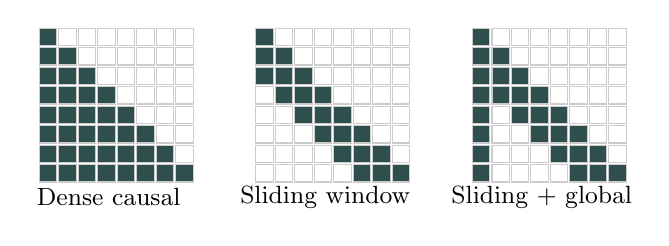
\begin{tikzpicture}[scale=0.55, every node/.style={font=\small}]
  % --- Mask 1: dense causal (for reference) ---
  \begin{scope}[shift={(0,0)}]
    \foreach \i in {0,...,7} {
      \foreach \j in {0,...,7} {
        \ifnum\j>\i\else
          \fill[DarkSlateGray] (\j*0.45, -\i*0.45) rectangle ++(0.4, -0.4);
        \fi
        \draw[gray!40] (\j*0.45, -\i*0.45) rectangle ++(0.4, -0.4);
      }
    }
    \node at (1.6, -3.9) {Dense causal};
  \end{scope}
  % --- Mask 2: sliding window w=2 ---
  \begin{scope}[shift={(5,0)}]
    \foreach \i in {0,...,7} {
      \foreach \j in {0,...,7} {
        \ifnum\j>\i\else
          \pgfmathtruncatemacro{\diff}{\i-\j}
          \ifnum\diff<3
            \fill[DarkSlateGray] (\j*0.45, -\i*0.45) rectangle ++(0.4, -0.4);
          \fi
        \fi
        \draw[gray!40] (\j*0.45, -\i*0.45) rectangle ++(0.4, -0.4);
      }
    }
    \node at (1.6, -3.9) {Sliding window};
  \end{scope}
  % --- Mask 3: sliding + global (token 0 attends/attended-to everywhere) ---
  \begin{scope}[shift={(10,0)}]
    \foreach \i in {0,...,7} {
      \foreach \j in {0,...,7} {
        \ifnum\j>\i\else
          \pgfmathtruncatemacro{\diff}{\i-\j}
          \ifnum\diff<3
            \fill[DarkSlateGray] (\j*0.45, -\i*0.45) rectangle ++(0.4, -0.4);
          \else
            \ifnum\j=0
              \fill[DarkSlateGray] (\j*0.45, -\i*0.45) rectangle ++(0.4, -0.4);
            \fi
          \fi
        \fi
        \draw[gray!40] (\j*0.45, -\i*0.45) rectangle ++(0.4, -0.4);
      }
    }
    \node at (1.6, -3.9) {Sliding + global};
  \end{scope}
\end{tikzpicture}
\caption{Three fixed-pattern sparse attention masks (causal, lower
triangular). Filled cells are computed; empty cells are skipped. Adding a
few ``global'' columns (right) recovers most long-range dependencies at
linear cost.}
\end{figure}

\section{What fixed-pattern sparse gives up}

The asymptote falls from \(\bigO(n^2)\) to \(\bigO(n)\). What is sacrificed?

\begin{itemize}
\item \textbf{Content-blindness.} The same set of attention pairs is used
for every input. ``Attend to position \(i \pm w\)'' is fast, but if the
relevant token is at distance \(2w\), the model has to relay information
through intermediate layers — possibly many of them.
\item \textbf{Theoretical expressivity holes.} Some tasks (associative
recall over arbitrary distances, exact-position retrieval) provably
require either dense or content-routed attention; sliding windows alone
cannot express them in a constant number of layers.
\item \textbf{Brittleness to long-range surprises.} A 100K-token document
might contain a single critical sentence at any position. Sliding windows
will miss it; global tokens are a partial fix but require knowing in
advance which positions matter.
\end{itemize}

In practice, fixed-pattern sparse + global tokens is the workhorse of
production long-context transformers (Mistral SWA, Llama 3 with extended
context, every encoder-only long-document model). It is not the bet of
this book's last chapter — that bet is on \emph{content-dependent}
sparsity (Chapter~\ref{ch:ssa}) — but it is the baseline against which
content-dependent sparsity has to justify itself.

\keyidea{Fixed-pattern sparse attention buys \(\bigO(n)\) by deciding the
sparsity pattern in advance, based only on position. Routing is content-
blind. The asymptote is gorgeous; the failure mode is missing the one
sentence in a million-token document that actually matters.}

\fillme{FILL-12-01}{Worked example: Longformer's effective receptive field after \(L\) layers}{%
  For sliding-window-only attention with window \(w\) and \(L\) layers,
  derive the effective receptive field of the top layer (it composes
  approximately like a convolution: \(L \cdot w\)). Plug in Mistral 7B
  numbers (\(w = 4096\), \(L = 32\)) and compute. Then explain in one
  paragraph why ``effective'' is a friendly word here: information from
  position 0 has to be relayed through 32 LayerNorms to reach the top
  layer, and quality decays.}{%
  Beltagy et al.\ 2020; Jiang et al.\ 2023 (Mistral 7B).}{%
  Half a page; one inline equation.}

\fillme{FILL-12-02}{Code listing: sliding-window attention in PyTorch}{%
  ${\sim}25$-line listing implementing causal sliding-window attention with
  window \(w\), without materialising the full \(n \times n\) score matrix.
  Use \texttt{torch.nn.functional.unfold} or a chunked loop. Comment on
  shape at every line. Below: one paragraph noting that \texttt{flash-attn}'s
  built-in sliding-window kernel is the production version.}{%
  Mistral 7B paper; \texttt{flash-attn} library docs.}{%
  ${\sim}25$ lines of code + one paragraph.}
